\subsection{Control Methods}\label{sec:control}
    \begin{figure}[H]
        \centering
        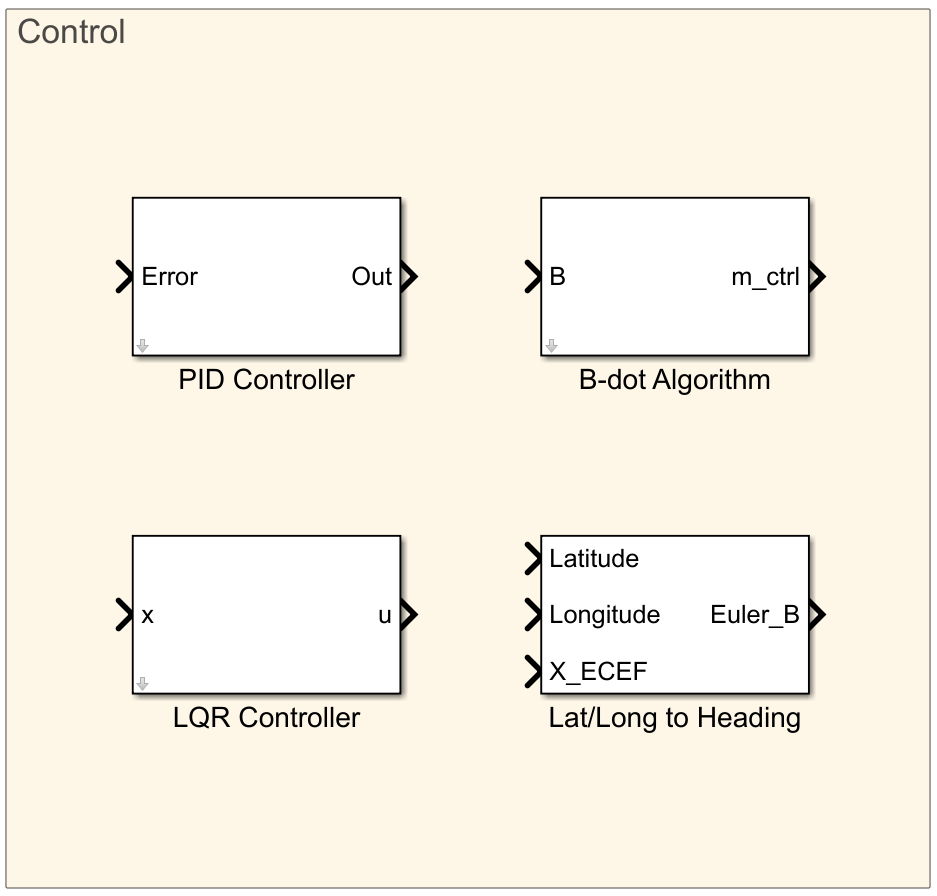
\includegraphics[width=0.7\textwidth]{2-toolbox/control.png}
        \caption{All Control blocks available in SCARS Parts Library}
        \label{fig:control}
    \end{figure}
    % \dots\textit{introduction}\dots
    In following sections all control methods implemented in \ac{scars} are described, along with their implementation. Furthermore, the tools available in the toolbox are presented. 
    
    \subsubsection{PID Controoler}
        % \dots\textit{finish description}\dots

        \ac{pid} is a feedback control loop method, widely used in most industrial applications where the simplicity of the design in of importance. It can be described with a transfer function in Laplace domain, as seen on \autoref{eqn:pid}
        
        \begin{equation}
            L(s) = K_p + \frac{K_i}{s} + K_d s
        \end{equation}\label{eqn:pid}

        Where $K_p$, $K_i$ and $K_d$ are, respectively, proportional, integral and derivative gains of the controller. Most relevant use of the PID controller is to minimize the error between reference state and actual state of the plant it controls - in case of \ac{scars} most often it will be used to provide input signals for the actuators, whether it is required thrust or moment, or in more specific cases, driving voltage.

        The controller can be set up to be only proportional, integral or derivative controller, or any combination of these modes. In that case, the gain values for unused modes have to be set to zero.

        In \ac{scars} the input of PID Controller block is error signal and the output is control signal. Only out The integral part is set to reset  
    
    \subsubsection{LQR}\label{sec:lqr}
        % \dots\textit{description}\dots
        \ac{lqr} is an optimal control method that uses a solution which in simplest form minimizes the quadratic cost function presented in \autoref{eqn:lqrcost} to generate static gain matrix $K$.

        \begin{equation}
            cost = \int{x^TQx+u^TRu}
        \end{equation}\label{eqn:lqrcost}
        
        \ac{lqr} method requires the state ($Q$) and control ($R$) weighting matrices, which respectively correspond to state and input vectors of the system. They describe the control effort that the controller puts on either minimizing the error in each state or magnitude of each input. Both $Q$ and $R$ matrices are diagonal, and most often are chosen arbitrarily and tuned in iterative process to achieve required controller behavior. Once calculated, the static gain matrix $K$ is used in a feedback control law:

        \begin{equation}
            u = -Kx
        \end{equation}

        To use \ac{lqr} method in \ac{scars} Toolbox, the state-space system of the spacecraft model has to be found first. As mentioned before, this is done by following the linearization process described in \autoref{app:linearization}.

        Implementing LQR Controller in \ac{scars} toolbox automates the process for the user, asking only to input $Q$ and $R$ matrices as block's mask parameters. The gain matrix is then calculated with MATLAB \verb|lqr| function.

        % \dots\textit{create the block and describe the implementation}\dots
        %https://www.mathworks.com/videos/trim-linearization-and-control-design-for-an-aircraft-68880.html

    \subsubsection{B-dot Algorithm}\label{sec:bdot}
        B-dot algorithm is popularly used for spacecraft detumbling. In its principle, magnetorquers are used to generate a torque that dampens the initial rotation of the spacecraft. The required magnetic moment is proportional to the change of magnetic field around the spacecraft. The required magnetic dipole $M$ is calculated from the following equation:

        \begin{equation}
            M = -k\dot{B}
        \end{equation} 

        Where $k$ is the tunable control constant and $B$ is the magnetic field intensity in satellite body frame\cite{capo2014b}.

    % \subsubsection{Quaternion Feedback Control}
    %     \dots\textit{description}\dots
        % Look into the topic
    
    % \subsubsection{Analisys Tools}
        % \dots\textit{description}\dots
        % As mentioned before, models built with \ac{scars} Toolbox are easily linearizable with Simulink Linear Analysis Tool. The process is described in \autoref{app:linearization}. 